\documentclass[conference]{IEEEtran}
\IEEEoverridecommandlockouts
% The preceding line is only needed to identify funding in the first footnote. If that is unneeded, please comment it out.
\usepackage{caption}
\usepackage{subcaption}
\usepackage{cite}
\usepackage{amsmath,amssymb,amsfonts}
\usepackage{cleveref}
\usepackage{algorithmic}
\usepackage{graphicx}
\usepackage{textcomp}
\usepackage{xcolor}
\usepackage{siunitx}
\def\BibTeX{{\rm B\kern-.05em{\sc i\kern-.025em b}\kern-.08em
    T\kern-.1667em\lower.7ex\hbox{E}\kern-.125emX}}

\def\proj{{\textbf{AILARON\ }}}
\def\proje{{\textbf{AILARON}}}
\newcommand{\cmt}[1]{{\color{red}{#1}}}

\begin{document}

% \title{Towards a system for Adaptive sampling of processes floating
%   with the current*\\
\title{Towards BioMapping: Autonomous Exploration of water column Biomass\\
% {\footnotesize 
% Towards BioSLAM: Autonomous Exploration for water column Biomass\\
% Towards BioSTAM: Simultaneous Tracking and Mapping of water column Biomass\\
% Towards BioLagranMap: Autonomous Lagrangian mapping of Biomass\\
% Spatio-Temporal Mapping and Exploration of water column Biomass\\
% Specie-Spatio-Temporal Mapping of water column plankton\\
% }
%\thanks{Identify applicable funding agency here. If none, delete this.}
}

\author{\IEEEauthorblockN{
Andreas V{\aa}ge\IEEEauthorrefmark{1},
Aya Saad\IEEEauthorrefmark{1},
Tor Nordam\IEEEauthorrefmark{2},
Annette Stahl\IEEEauthorrefmark{1},
Martin Ludvigsen\IEEEauthorrefmark{3},
Kanna Rajan\IEEEauthorrefmark{4},
}
\IEEEauthorblockA{\IEEEauthorrefmark{1}
\textit{Dept. of Engineering Cybernetics},
\textit{Norwegian University of Science and Technology (NTNU)},
Trondheim, Norway \\
}
\IEEEauthorblockA{\IEEEauthorrefmark{2}
\textit{Dept. of Environment and New Resources},
\textit{SINTEF Ocean},
Trondheim, Norway \\
}
\IEEEauthorblockA{\IEEEauthorrefmark{3}
\textit{Dept. of Marine Technology},
\textit{NTNU},
Trondheim, Norway \\
}
\IEEEauthorblockA{\IEEEauthorrefmark{4}
\textit{Underwater Systems and Technology Laboratory},
\textit{ University of Porto},
Porto,  Portugal \\
}
}
\maketitle

% \begin{abstract}

% \end{abstract}

\begin{IEEEkeywords}
AUV, Machine Learning, Adaptive Sampling, Gaussian Process, Plankton imaging
\end{IEEEkeywords}

\section{Introduction and Motivation}

Planktonic biomass forms the fundamental food source for consumers at
higher trophic levels. They play a significant role in producing more
than $50\%$ of the global oxygen supply. Hence, studying their
community structure, abundance, and dispersion across the ocean is a
primary research concern. To avoid transferring planktonic organisms
to the lab or applying ship-based point profiling as traditional
approaches suggest our project, \proj (\textbf{A}utonomous
\textbf{I}maging and \textbf{L}earning \textbf{A}i \textbf{RO}bot
identifying pla\textbf{N}kton taxa in-situ), an open source AUV
framework that images, identifies, and measures targeted plankton
spatial spread in-situ, akin to a ``sniffer dog''. If successful, researchers can specify a search area, a set of plankton classes of interest and launch the AUV from shore. The AUV then performs an initial rough search over the area and adaptively maps the found targeted biology over time. At the end of the
day the AUV returns to shore where it remotely is controlled in and picked up.

In this paper we present the adaptive sampling algorithm, which based
on input from the on board imaging and deep learning classification
module, performs data processing using Gaussian Process (GP)
Regression combined with a 4D current model and uses the estimated
spatial distribution to perform intelligent path planning.

%\section{Motivation}

\section{Related Work}

In \cite{fossum18b} an AUV adaptivly measures Chlorophyll a to
estimate biomass 3D spatial structure, based on GP regression,
\cite{das15} used adaptive sampling to determine when optimally
perform water samples with an AUV.  However both assumes the sample
time-span is short enough for the temporal movement of the biomass
caused by the current to be ignored as noise.  \cite{smith10} used
ocean model predictions to plan glider paths to optimally sample algae
patches, but does not adaptivly update the path during the search.
Incorporating the current into the adaptive sampling is ambitious, but
numerical ocean models provides more accurate forecasts and small and
improved acoustic sensors allows AUVs to directly measure local
current profiles \cite{Fong2006, Cusi2017}.

\section{Technical Description}

A overview of the information flow can be seen in
\cref{fig:sensePlanActLoop}. When plan generation and execution embedded on a robot is continuous, sensing of the robots environment
updates the internal representations which could modify future actions
with plan synthesis and in turn future actions.  In enabling this
continuous \textbf{sense}, \textbf{plan} and \textbf{act} loop, the
robot can adapt to changing conditions in the real world enabling a
cognitive capacity that most robotic vehicles to date, fall short of
\cite{rajan12}.

\begin{figure}[tbp]
% \centerline{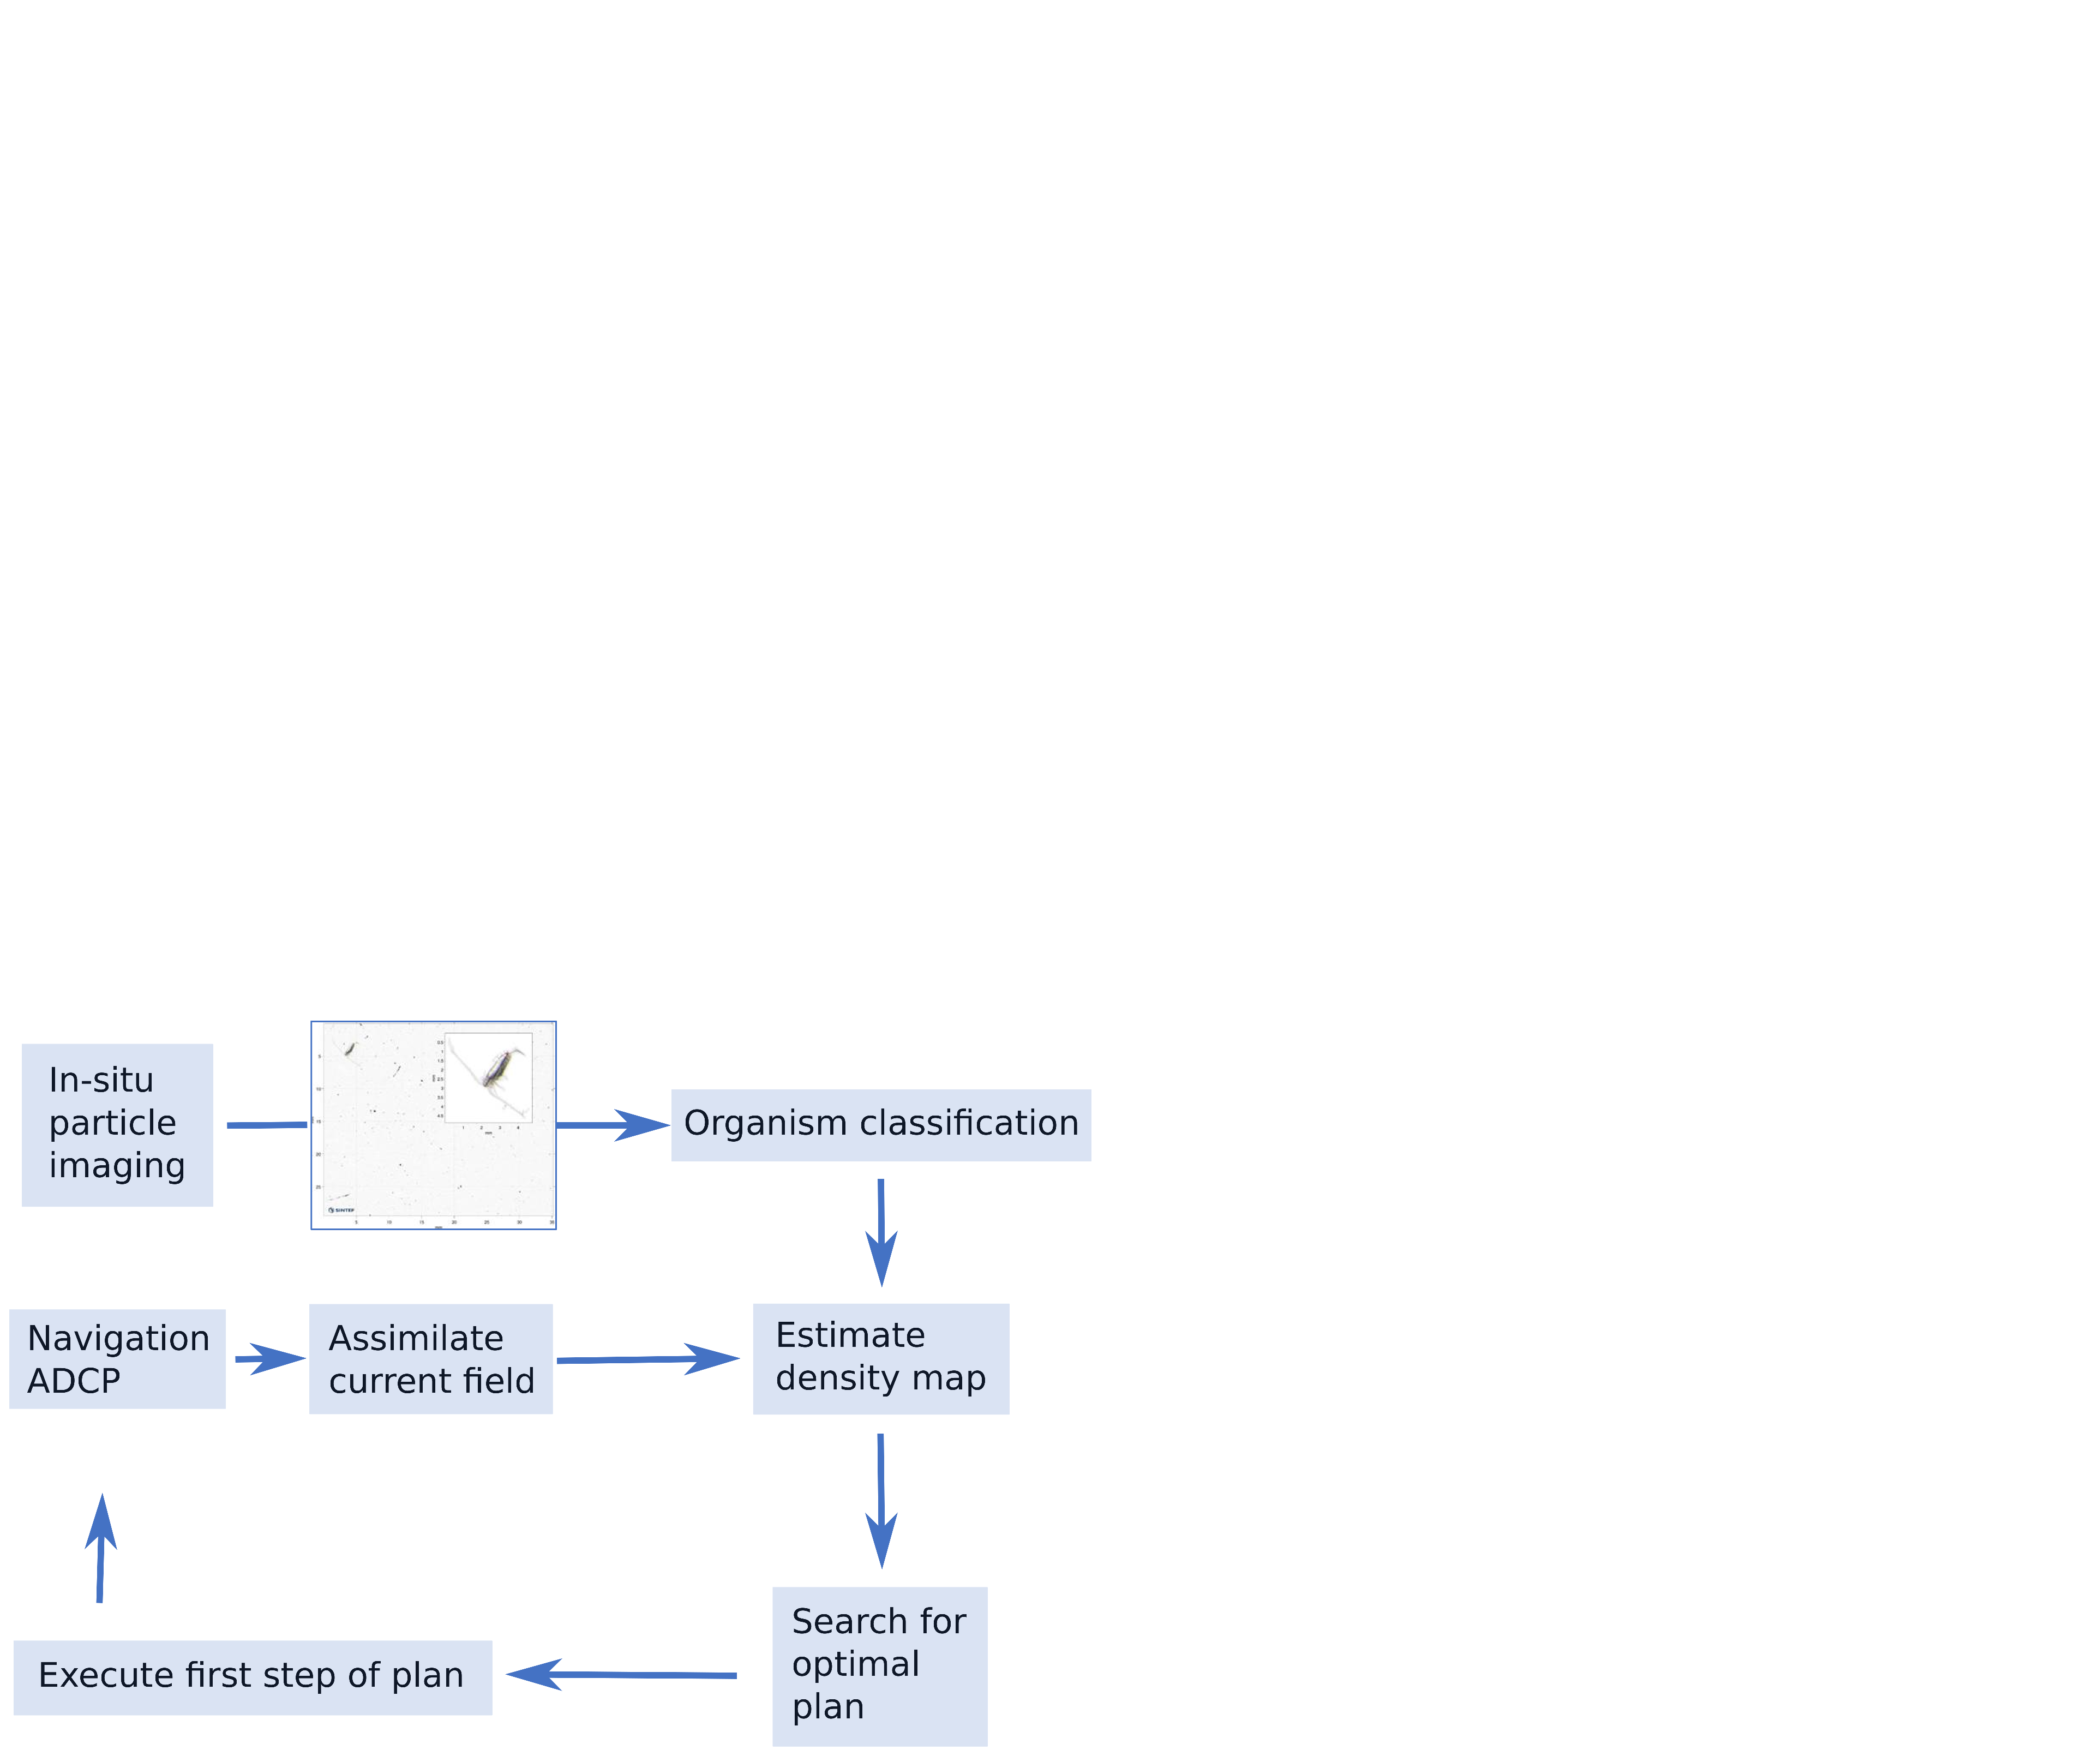
\includegraphics[width=0.8\linewidth]{figures/workflow-simplified.eps}}
\centerline{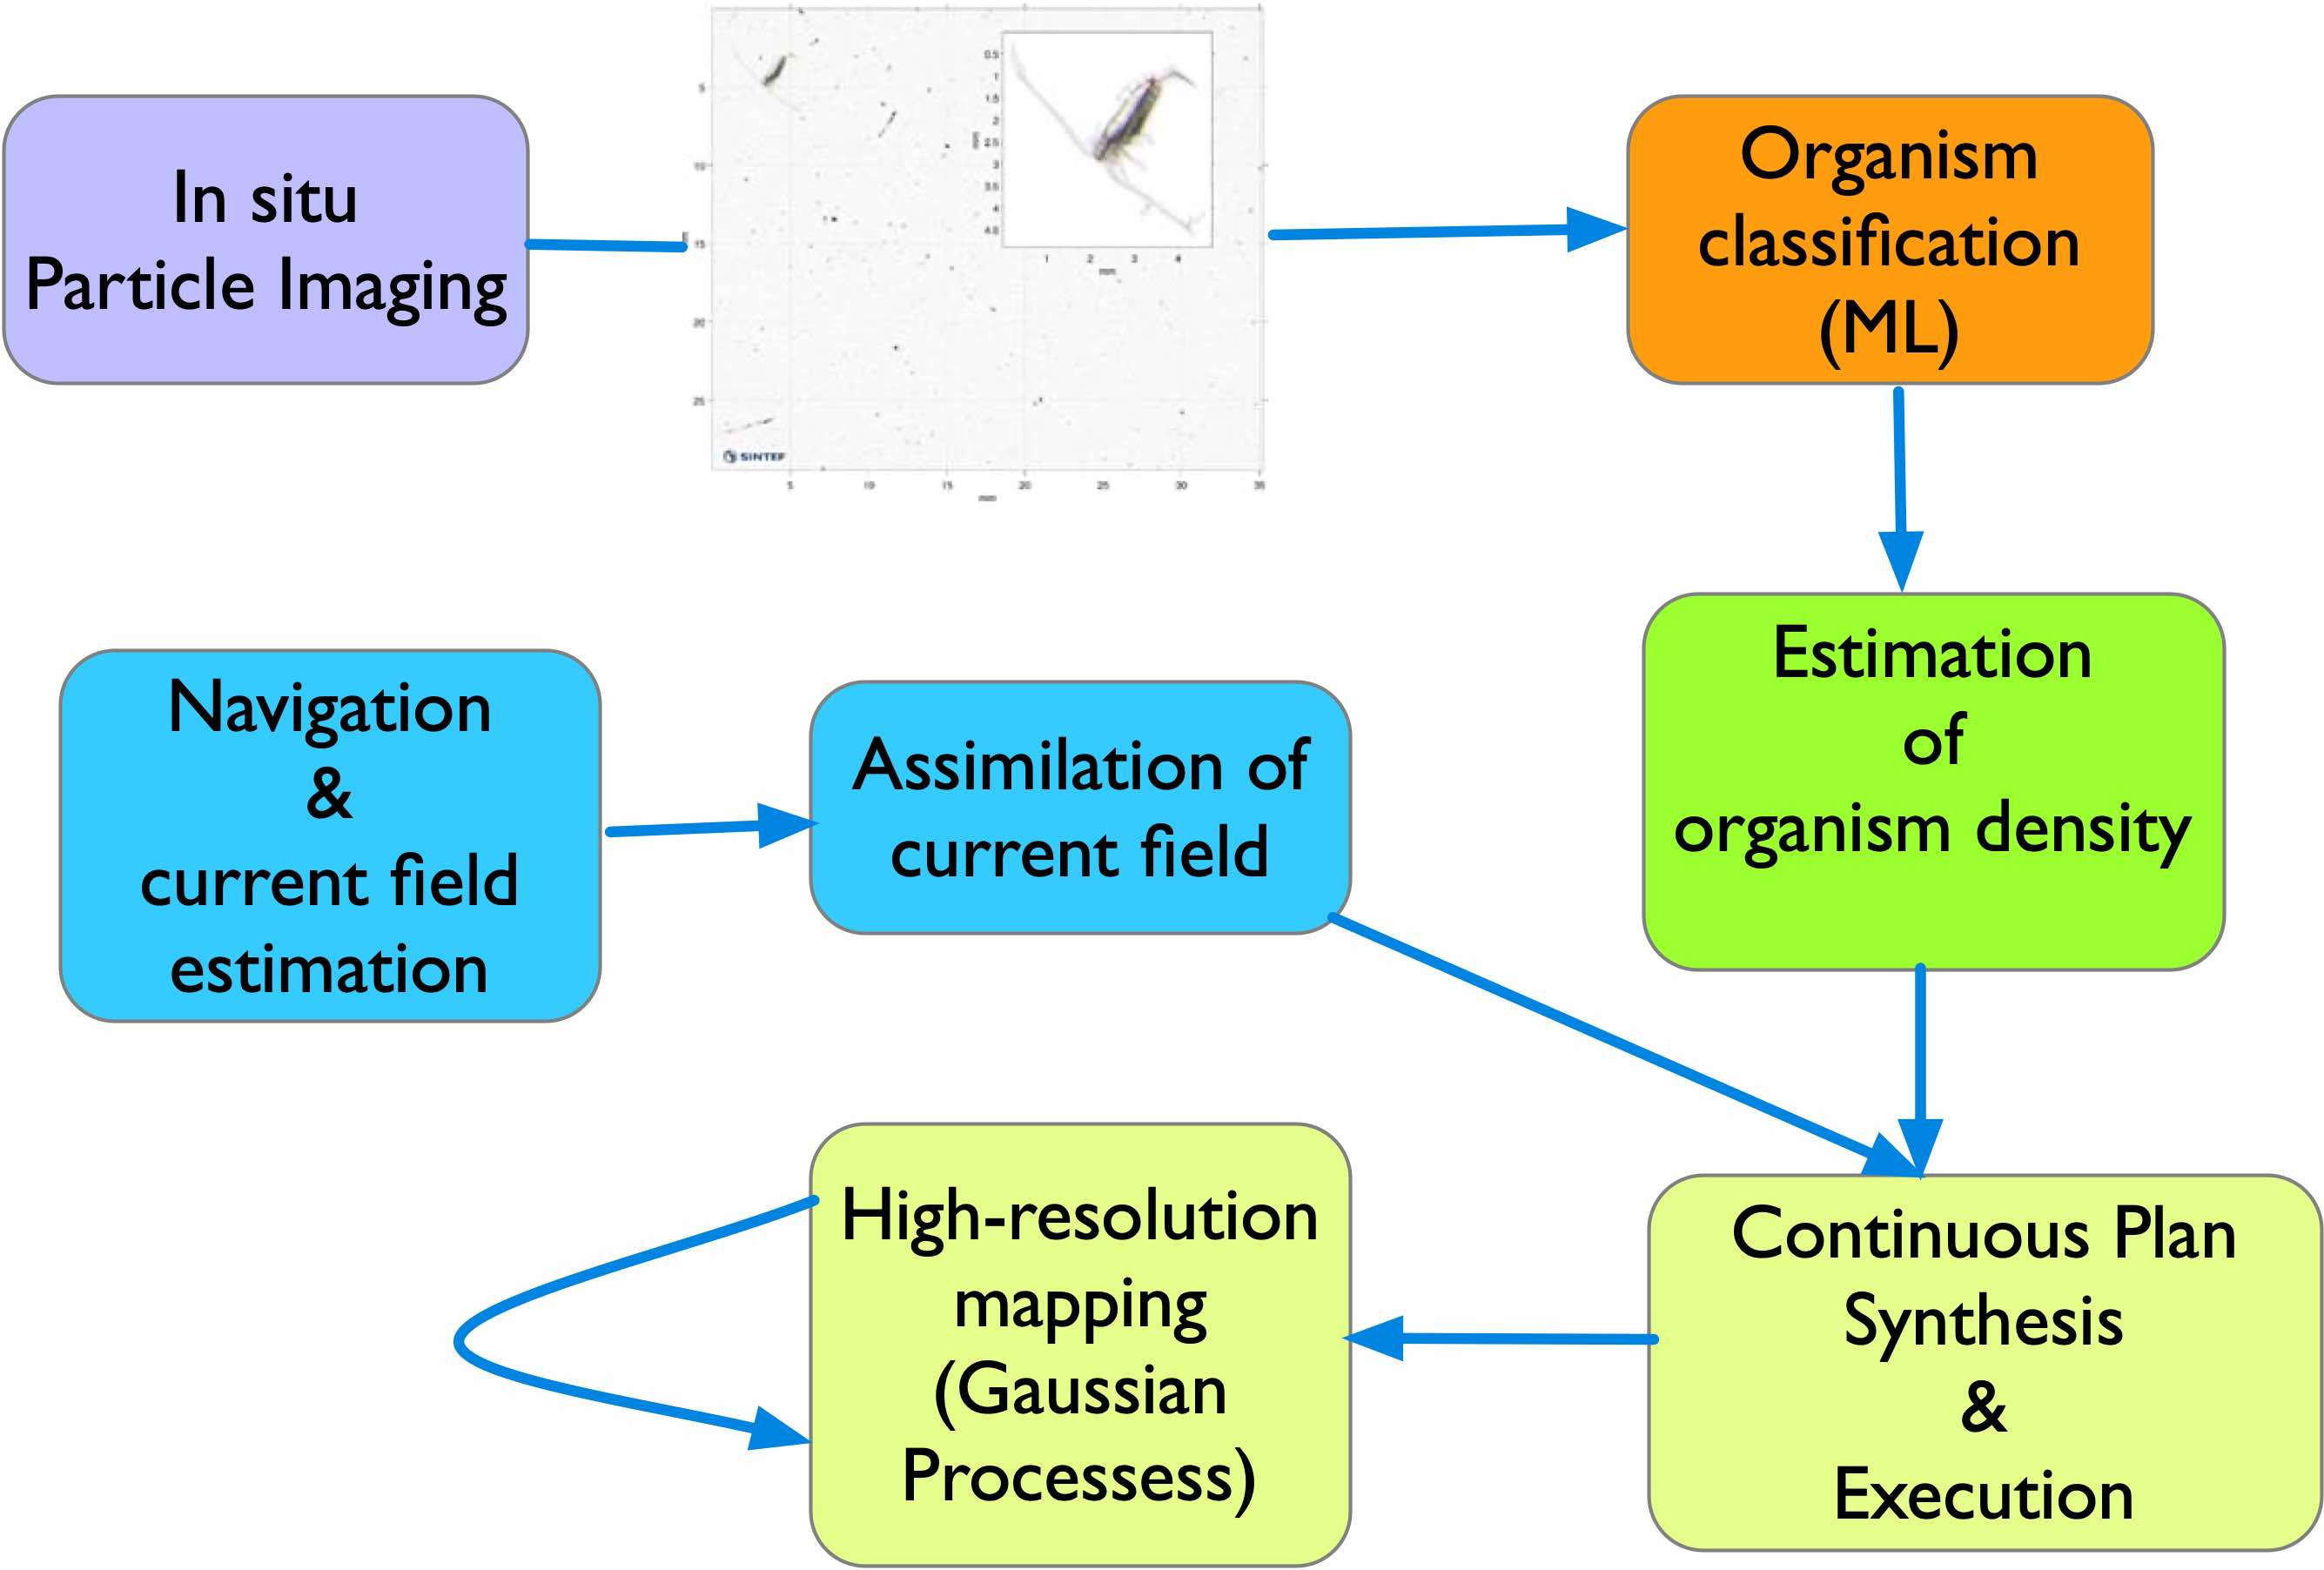
\includegraphics[width=0.8\linewidth]{figures/workflow-simplified.jpg}}
\caption{The overall information flow on board the AUV in \proje. After accumulating the measurements into the models, a plan for further data collection is found. The AUV will then start executing the plan, and thus gather new measurements which again are used to update the plan.}
\label{fig:sensePlanActLoop}
\end{figure}

\subsection{Particle detection-classification pipeline}

A novel imaging camera \cite{Davies2017a} based on a transmittance
imaging system, is embedded into the hull of the AUV. This onboard
imaging enables in-situ time-series capturing of magnified images of
particles floating through an installed volume of \SI{55}{\micro\meter}
diameter.

This stream of captured images is, in turn, input to object detection
and classification pipeline that adopts deep machine learning (DL)
approaches. The pipeline line starts with extracting and identifying
the set of objects per image frame in the time-series. Then extracted
objects are input to a classification module for further taxa
identification and recognition by means of an embedded DL
architecture.

We exerted a thorough performance comparison between state-of-the-art
DL architectures. Our selection criteria recommend the use of a simple
5-convolutional-layers network since it outperforms the other DL
structures in terms of prediction speed, detection accuracy, and space
in the memory. The accuracy achieved after training the network over a
dataset of 7800 different images of planktonic organisms was $95.09\%$
compared to $93.54\%$,$93.54\%$, $91.98\%$, $92.24\%$, $91.21\%$, and
$82.68\%$ achieved by Zooplanktonet \cite{dai2016zooplanktonet},
VGGNet \cite{simonyan2014very}, ResNeXt \cite{xie2017aggregated},
ResNet \cite{he2016deep}, AlexNet \cite{krizhevsky2012imagenet} and
GoogleNet \cite{szegedy2015going} respectively.

%The novel SILCAM has been implemented into the hull of an AUV.
%It continuously captures magnified images of particles floating trough its capture volume.
%The raw images are processed and classified by a state-of-the-art deep learning model on-board the AUV, resulting in a stream of detected particle classes along with prediction confidences.
Measurements of the different classes
concentration, along with their corresponding variances, are inferred from the classification,
and they are provided as an output of this process.
%For now we only consider one feature at a time, i.e. the total concentration of particles, but extending the system to multiple classes is possible.
%Also other observable processes then microbial biology could be monitored with the same system.

\subsection{Spatio-Temporal modelling}
%As the spatial density of microbiology is not stationary, but changes over time we model it as spatio-temporal process.
To enable mapping microbiological processes over time as they float
with the current a local current model is used to predict the temporal
movement of the biomass, then Gaussian Process Regression/Kriging is
used to estimate a dense spatial distribution of the biomass.

\paragraph{Local Current Model}
Represented as a 4D (space and time) vector field over the operational
area of the AUV, it is either generated prior to missions based on a
numerical hydrodynamic model
%SINMOD \cite{slagstad2005}
or accumulated during the mission from acoustic doppler current
profiler (ADCP) measurements on the AUV.  A Lagrangian particle
transport model, derived from previous and ongoing work at SINTEF
\cite{Rye2006}, is run onboard the vehicle.  Particles are transported
individually, using a variable-time step
integrator %\cite{Dormand1980}
through the current field, applying a random walk with the local
diffusivity.

\paragraph{Gaussian Process Regression} 
Gaussian Process Regression is performed over the particles to estimate the spatial structure of the microbiology concentrations.
%Gaussian process regression is data driven and requires very few parameters, which is important as the process observed is little known, making it hard to fit a parameter based model.
In addition to estimating the mean predicted values (the Kriging surface)
Gaussian Process regression also estimates the uncertainty, which is
later used to balance exploration vs exploitation when deliberating
where the AUV should go next.

%(\cmt{Cite. This is confusing; are you using a GP with the hydro-dynamic flow? I suspect what you want to say is, once a hot-spot has been identified, then to understand its spatial structure (size, extant and potentially as a result, the community (of the micro-organism) structure), one needs to do a GP (a la, work in Runde). Right?})
\subsection{Path Generation with Heuristics}
The search for a path which maximises a given objective function based on the estimated GP model/Kriging surface, is made more efficient by utilising traditional survey paths as heuristics. E.g the standard square survey showed in
Fig.~\ref{fig:munkholmen} is parameterised by the covered rectangle
and its density, which is significantly fewer parameters to optimise
compared to specifying each line individually.
%Bresenham's line algorithm

The objective function is calculated over the estimated GP model along
the path candidate. It is based on a combination of the following interests:
\begin{itemize}
    \item Scientific interest in particular plankton classes. 
    \item Exploitation: maximise expected measured concentration per travelled distance
      according to the kriging surface. 
    \item Exploration: minimise model variance per travelled distance by sampling from
      previously little visited areas.
    \item Lagrangian Tracking: Follow the biomass by following the estimated current.
\end{itemize}
%(\cmt{This is very abrupt. You want to say where the GP is being used, but after you talk about the plan-exec, since it is the plan-exec component which determines when to activate the GP and modify the kernel. There should be a nice flow between when you introduce the GP with the rest of the para's below. And after Plan/Exec.}).
All code is open source and based on open source projects. Including
the AUV control and navigation software (DUNE) and mission control
(Neptus)\cite{pinto2013lsts}.

\section{Experimental Results}

The system is being tested and developed in simulations and on historic
data.
The simulator is based on a numeric hydrodynamic model and is overall
very similar to the estimation system on board the AUV, only larger scale.
GP kernels, learned from historic data, are used to draw new simulated biomass which the simulated AUV draws measurements from. 
Fig.~\ref{fig:munkholmen} shows the planned path based on historic
data from a survey in the Trondheim fjord in April 2020, during an
annual algae bloom. The planned path is maximising the expected
concentration of detected algae, while also minimising the variance of
the estimated Gaussian process.
\cref{fig:Simulation} shows a larger simulation run from the same area, where the initial biomass concentration were extrapolated from the historic data.

\begin{figure}[htbp]
  \centering
  \includegraphics[width=\linewidth]{figures/LAUV.jpg}
  \caption{The Light Autonomous Underwater Vehicle (LAUV)
    \emph{Roald}, used in \proje. The sample volume of the SILCAM,
    capable of capturing images of microbial biology, can be seen on
    the underside of the nose. The equipped Doppler Velocity Logger
    include current profiling capabilities used to assimilate a
    current field during operation.}
  \label{fig:roald}
\end{figure}

\begin{figure}[htbp]
  \centering
  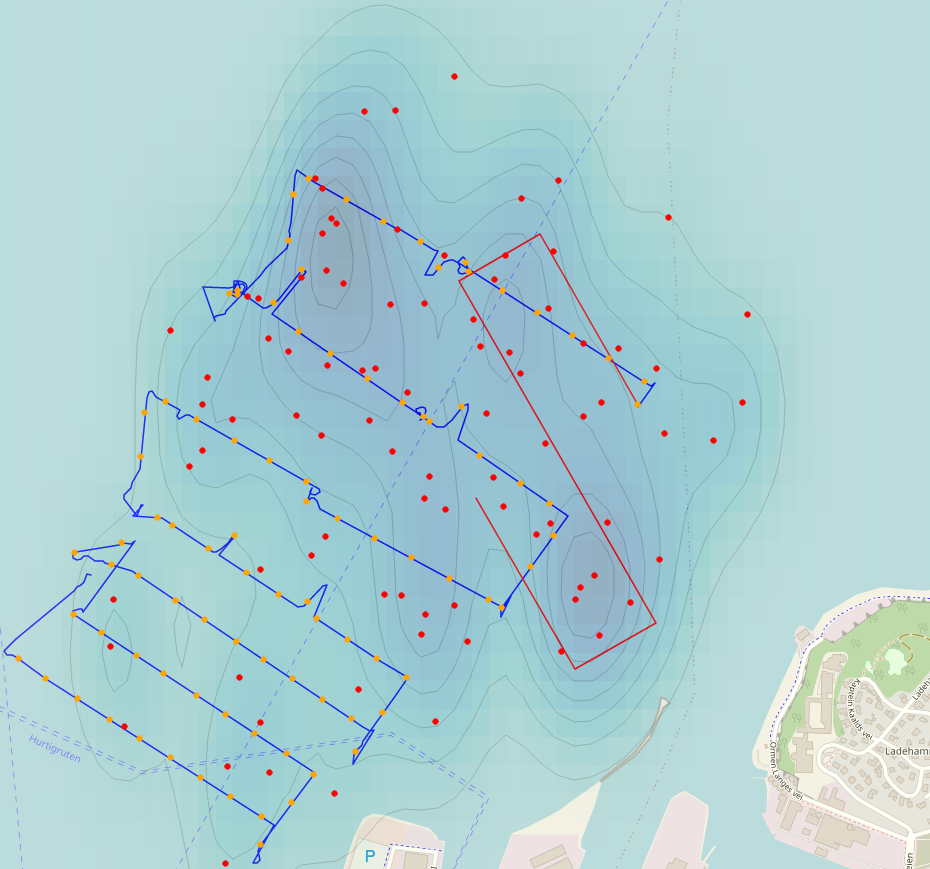
\includegraphics[width=\linewidth]{figures/munkholmen_planned_path.png}
  \caption{Historic data. The AUV has traversed the blue path and gathered data (orange points), which has been transported with the current, and are now
    estimated to be located at the red points.  The contour shows the
    predicted concentration for which the red path is maximizing
    expected measured concentration and minimising model variance per travelled distance.}
  \label{fig:munkholmen}
\end{figure}

\begin{figure}[t]
     \centering
     \begin{subfigure}[htb]{\linewidth}
         \centering
         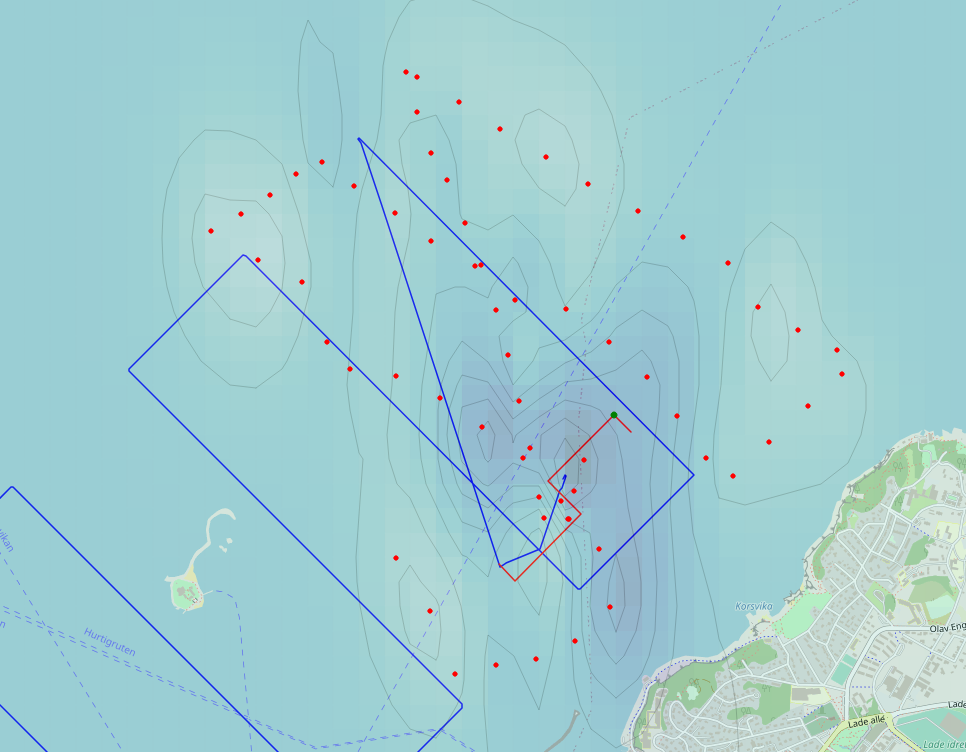
\includegraphics[width=\textwidth]{figures/sim-estimate.png}
         \caption{The contour shows the estimated concentration. The red path shows the chosen lawn-mover path used as a heuristic for speeding up the path search, and the blue shows the actual travelled path. The red points shows the predicted position of measurements which are fresh enough to still be taken into account.}
         \label{fig:sim-estimation}
     \end{subfigure}
     \\
     \begin{subfigure}[htb]{\linewidth}
         \centering
         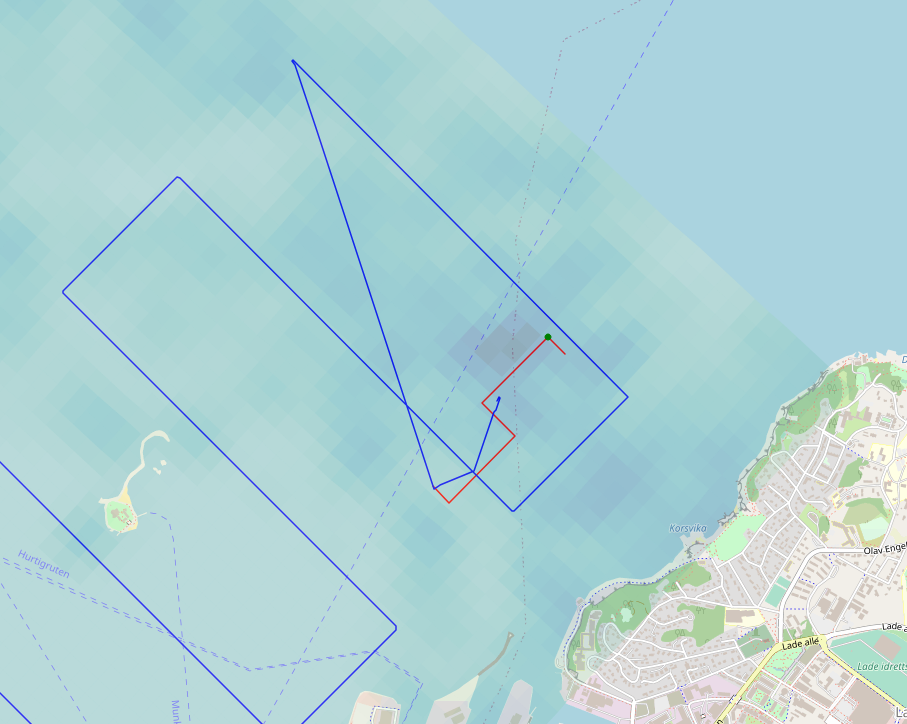
\includegraphics[width=\textwidth]{figures/sim-gt.png}
         \caption{The simulated biomass concentration from which the measurements are drawn. Ground truth is one of benefits from working with simulations.}
         \label{fig:sim-gt}
     \end{subfigure}
        \caption{Simulation results of a larger survey where the AUV first followes a predetermined lawn-mover path, then adaptively locates and sample measurements from the largest hot-spot.}
        \label{fig:Simulation}
\end{figure}

%Future steps include experimentation with the AUV operating autonomously in open waters.

% \section*{Acknowledgment}
% This work was supported by the Research Council of Norway through the FRINATEK/IKTPLUSS program, project number 262701.

\bibliographystyle{IEEEtran}
\bibliography{references}


\end{document}
